\documentclass{article}
\usepackage[utf8]{inputenc}
\usepackage{booktabs}
\usepackage{graphicx}
\usepackage{float}
\usepackage[section]{placeins}
\renewcommand{\thesubsection}{\thesection.\alph{subsection}}
\usepackage{natbib}
\usepackage[shortlabels]{enumitem}

\title{Tarea 3: Modelo Relacional}
\author{Arteaga Hernández Alejandro Iabin \and
Barocio Gomez Luis Fernando \and
Castrejón Estrada Juan Carlos \and
Ledesma Granados Roberto Andrés }

\date{Abril 2020}

\begin{document}

\maketitle
\section{Preguntas de repaso}
\begin{itemize}
    \item ¿Qué es una relación y qué características tiene?\\
    Una relación $R$ de los conjuntos $A_1, A_2, ..., A_n$ es un subconjunto del producto cartesiano de los conjuntos: $R \subseteq A_1 \times A_2 \times ... \times A_n$. Características: 
    \begin{itemize}
        \item No hay tuplas repetidas.
        \item El orden de las tuplas no es importante.
        \item Los atributos están desordenados.
        \item Los atributos tienen valores atómicos.
    \end{itemize}
    \item ¿Qué es un esquema de relación? \\
    Describe la estructura y las restricciones de los datos que se representan en un dominio particular. Puede describirse como un esquema de una base de datos que describe la forma en que los datos se organizan en tablas. Este esquema no contendrá ningún tipo de datos. En un esquema relacional, cada tupla se divide en campos llamados dominios.
    \item ¿Qué es una llave primaria?, ¿qué es una llave candidata?, ¿qué es una llave mínima?, ¿qué es una super llave?
    \begin{itemize}
        \item Llave primaria: La llave que permite identificar tuplas de la relación de forma única.
        \item Llave candidata: Son llaves que no han sido escogidas como llaves primarias pero que también podrían identificar de manera única a una tupla.
        \item Llave mínima: Es un conjunto mínimo (irreducible) no vacío de atributos que identifican de manera única a cada tupla.
        \item Super llave: Atributo o conjunto de atributos que identifica de manera única una relación.
    \end{itemize}
    \item ¿Qué restricciones impone una llave primaria y una llave foránea al modelo de datos relacional? \\
    El problema de integridad referencial: la Base de Datos no debe contener valores de llave foránea que no se correspondan con un valor de la llave primaria (Si B referencia a A,entonces A debe existir).
    \item Investiga cómo se traducen las categorías (presentes en el modelo E/R) al modelo relacional. Proporciona un ejemplo. \\
    Si las superclases de la categoría tienen diferentes llaves primarias:
    \begin{enumerate}
        \item Se crea una tabla T que corresponda a la categoría y se le asigna una llave sustituta arbitraria.
        \item Se añade a la llave sustituta a modo de llave foránea en cada una delas tablas Ti que corresponden a las superclases de la categoría.
    \end{enumerate}
    Si las superclases de la categoría tienen la misma llave primaria:
    \begin{enumerate}
        \item Se crea una tabla T que corresponda a la categoría y se le asigna como atributo llave primaria la llave común a todas las superclases de la categoría.
    \end{enumerate}
    Ejemplo:\\
    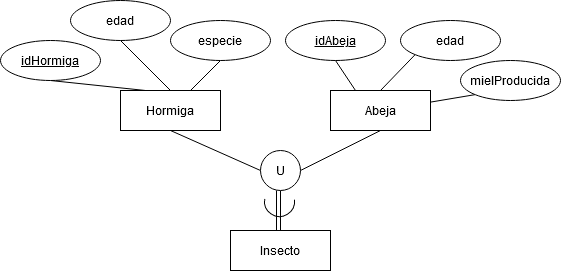
\includegraphics[scale=0.5]{ej.png} \\
    Hormiga(\underline{\textbf{IdHormiga}}, edad, especie, \textbf{idInsecto})\\
    Abeja(\underline{\textbf{IdAbeja}}, edad, mielProducida, \textbf{idInsecto})\\
    Insecto(\underline{\textbf{idInsecto}})\\
\end{itemize}
\section{Modelo relacional}
a)\\
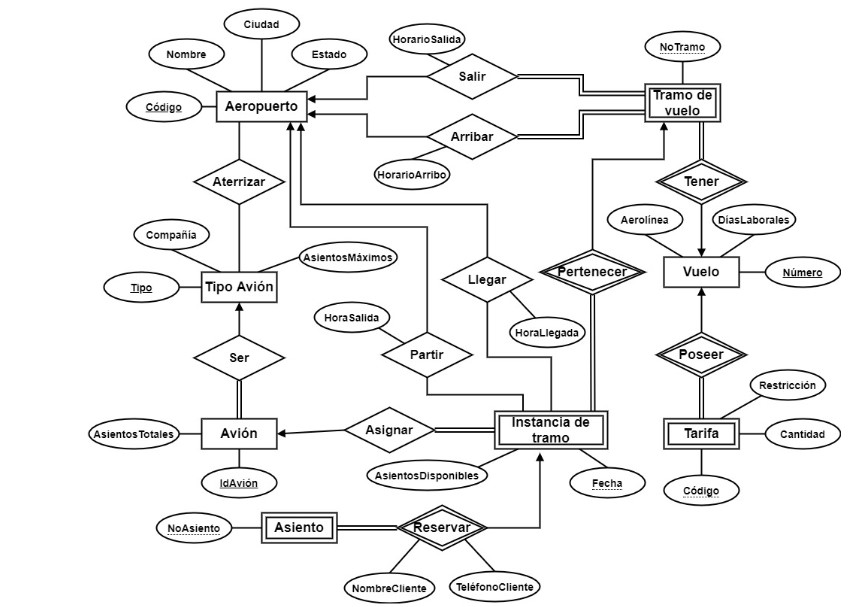
\includegraphics[scale=0.55]{aero.jpg} \\
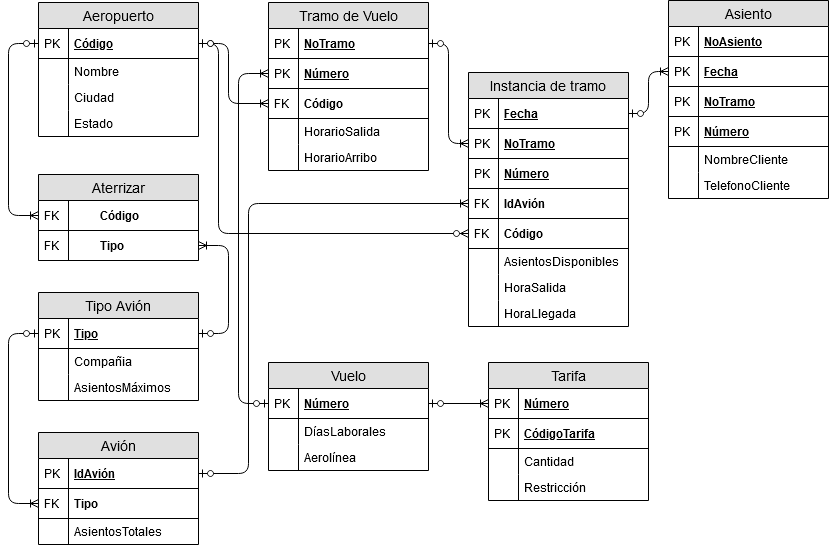
\includegraphics[scale=0.45]{aero.png} \clearpage
b)\\
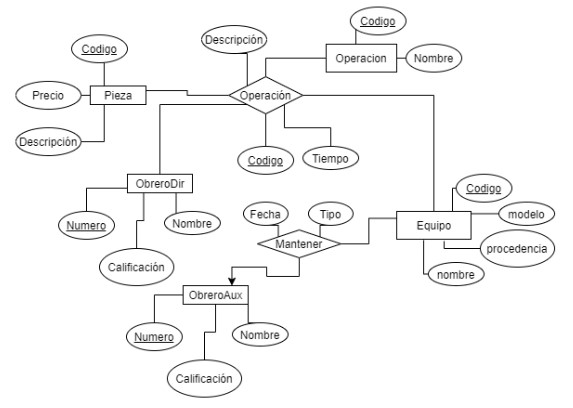
\includegraphics[scale=0.8]{fab.jpg} \\
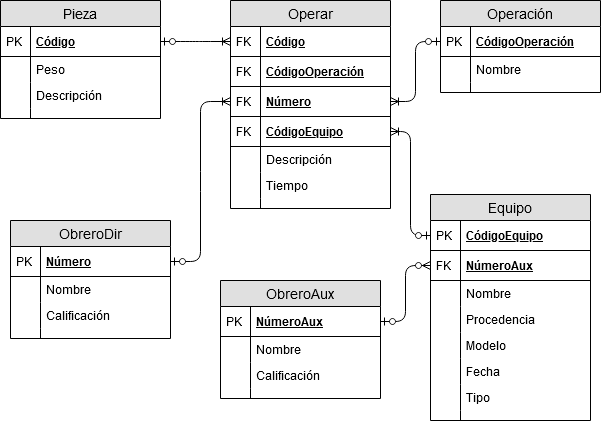
\includegraphics[scale=0.6]{fab.png} \\
\section{Modelo relacional e inserción de tuplas}
Considera el siguiente modelo \textbf{E/R}
\begin{figure}
    \centering
    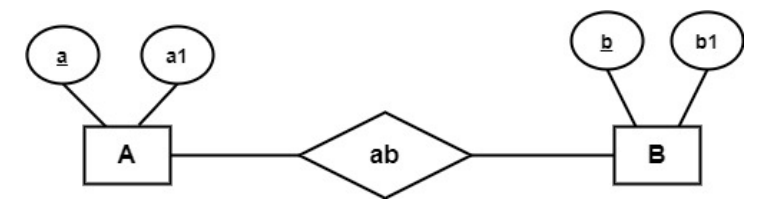
\includegraphics[scale=0.5]{tres.PNG}
    \caption{Modelo E/R}
    \label{fig:er}
\end{figure}


Completa la tabla que se presenta a continuación, convirtiendo el modelo E/R en un esquema relacional, para todas las opciones de cardinalidad. Escribe las relaciones y subraya su llave primaria: 


\begin{figure}[ht]
    \centering
    
\includegraphics[scale=0.7]{Capture.PNG}
    \caption{Modelo relacional}
    \label{fig:tabla}
\end{figure}

Supón que para la tabla que llenaste anteriormente se desea agregar algunas tuplas a las relaciones. Indica cuáles de las tuplas siguientes se pueden insertar en el esquema relacional que creaste para la relación M: N. Supón que agrega los elementos en el orden indicado a continuación y, que los atributos a y b son de tipo entero, mientras que a1 y b1 son de tipo cadena. A tiene cuatro tuplas identificadas por los valores 1, 2, 3 y 4. B tiene 5 tuplas identificadas por 10, 20, 30, 40, 50. Justifica tu respuesta:

\begin{itemize}
    \item \textbf{a. (1,10); (1,20); (2,10); (2,10); (3,40); (40,4)}
    \par
    (1,10), (1,20), (2,10) pueden ser ingresados sin problema, ya 
    que cumplen la relación muchos a muchos, pero (2,10) ya no puede
    ser ingresado porque el elemento (2,10) ya está y no puede haber 
    elementos repetidos, (3,40) es aceptado pero (40,4) es rechazado 
    porque no hay ningún elemento en A que sea 40
    
    \item \textbf{b. (2,40); (2,30); (5,10); (3,10); (3,40); (4,10)}
    \par
    (2,40), (2,30), son agregadas sin problemas, pero (5,10) no puede
    ser agregado ya que 5 no es una llave en A, (3,10), (3,40) y (4,10) se 
    agregan sin problemas
    
    \item \textbf{c. (1,10); (1,20); (2,20); (2,30); (3,10); (3,50)}
    \par
    (1,10), (1,20), (2,20), (2,30), (3,10), (3,50)
    son agregados sin problemas
    
    \item\textbf{ d. (10,1); (20,1); (10,2); (10,10); (40,3)}\par
    Todos los elementos serían rechazados porque el SMBD ya que ningún elemento de la izquierda pertenece al conjunto de llaves de A. 
\end{itemize}

¿Cuáles de las siguientes tuplas se pueden insertar en el esquema relacional que creaste para la relación \textbf{1:N}?
Considera el mismo escenario inicial para las relaciones A y B:

\begin{itemize}
    \item \textbf{a. (10,’A’,1); (20,’B’,2); (10,’C’,3); (30,’A’,4); (50,’M’,3)}
    \par 
    (10,’A’,1),(20,’B’,2) Si se pueden insertar en B(b,b1,a) que contiene la relación, (10,’C’,3) no se puede insertar porque la llave 10 ya fue insertada, (30,’A’,4); (50,’M’,3) si pueden ser insertados.
    
    \item \textbf{b. (1,10); (1,20); (2,20); (2,30); (3,10); (3,20)}
    \par (1,10), (1,20), (2,20), (2,30), (3,10), (3,20) no pueden ser insertados
    porque 1,2,3 no son llaves primarias en B
    \item \textbf{c. (1,’A’,10); (2,’B’,20); (3,’C’,30); (4,’A’,20); (1,’A’,40)} \par
    (1,’A’,10); (2,’B’,20); (3,’C’,30); (4,’A’,20); (1,’A’,40) No pueden ser
    insertadas, porque 1,2,3,4 no son llaves primarias en B
    \item \textbf{d. (10,’A’,1); (20,’B’,2); (30,’C’,3); (40,’A’,2)}
    \par
    (10,’A’,1); (20,’B’,2); (30,’C’,3); (40,’A’,2) Si pueden ser insertadas sin
    problemas porque, 10,20,30 y 40 sin son llaves validas en B y 1,2,3 también
    son llaves válidas en A
\end{itemize}
¿Cuáles de las siguientes tuplas se pueden insertar en el esquema relacional que creaste para la relación 1:1?\par
Considera el mismo escenario inicial para las relaciones A y B:
\begin{itemize}
    \item \textbf{a. (1,10); (1,20); (2,10); (2,10); (3,40); (40,4)}
    \par (1,10) se agrega, pero (1,20) ya no porque 1 ya está relacionado con 10, de igual manera (2,10) ya no porque 10 está ya relacionado con 1,
    (3,40) se agrega sin problemas pero (40,4) no porque 40 no es llave primaria en A
    \item \textbf{b. (40,1); (30,2); (50,3); (20,4)}
    \par (40,1); (30,2); (50,3); (20,4) No se agregan porque 40,30,50,20 no son llaves primarias en A
    \item \textbf{c. (1,10); (1,20); (1,30); (2,10); (2,20); (3,10)}
    \par (1,10) se agrega pero (1,20) no porque 1 ya está relacionado con 10,
    lo mismo para (1,30), (2,10) no se agrega porque 10 ya está relacionado con 1, (2,20) si se agrega y el (3,10) no porque 10 ya está relacionado.
    \item \textbf{d. (1,20); (2,30); (3,40); (4,50)}
    \par (1,20); (2,30); (3,40); (4,50) Todos son agregados sin problemas, ya que no hay llaves repetidas
\end{itemize}
\section{Modelo relaciones y restricciones de integridad}
A continuación, se encuentra el modelo relacional del departamento de recursos humanos de una empresa. En este esquema, supón que \textbf{desde} es inclusivo, mientras que \textbf{hasta} es exclusivo, definiendo el período \textbf{[desde,hasta)}.

\begin{itemize}
    \item \textbf{Departamento} (\textbf{\underline{depto\_num}}, depto\_nombre)
    
    \item \textbf{Trabajar} (\underline{\textbf{emp\_num}}, \underline{\textbf{depto\_num}}, \underline{\textbf{desde}}, hasta)
    
    \item \textbf{Administrar} (\underline{\textbf{emp\_num}}, \underline{\textbf{depto\_num}}, \underline{\textbf{desde}}, hasta)
    
    \item \textbf{Empleado} (\underline{\textbf{emp\_num}}, nacimiento, nombre, apellido, género, fecha\_contratación)
    
    \item \textbf{Salario} (\underline{\textbf{emp\_num}}, salario, \underline{\textbf{desde}}, hasta)
    
\end{itemize}

A partir del modelo relacional anterior, indica cuáles de las siguientes afirmaciones son verdaderas y por qué razón
(sin considerar restricciones adicionales):

\begin{enumerate}[a)]
    \item Dos departamentos con el nombre \textbf{‘Sistemas’} podrían existir al mismo tiempo\par
    Si, el campo depto\_nombre no tiene ninguna restricción
    
    \item Ningún empleado puede trabajar en un departamento y administrar otro al mismo tiempo. 
    \par Si pueden, las tablas trabajar y administrar son \textbf{ajenas} y pueden existir 2 iguales en las distintas tablas sin problema.
    
    \item Un empleado podría ser empleado en dos departamentos al mismo tiempo
    \par Si, puede ser empleado en distintos departamentos o incluso en el mismo con distintas fechas.
    \item Para las entradas en la relación \textbf{Administrar, hasta} no puede ser anterior a \textbf{desde}.
    \par se podría, no hay ninguna restricción que lo prohíba.
    
    \item Dado un empleado, podemos identificar exactamente un departamento donde trabaja.
    \par Si, podemos hacer una selección de las columnas donde esté el valor del número del empleado buscado y elegir un departamento. 
    
    \item Un empleado puede cobrar más de un salario al mismo tiempo.
    \par Sí, si trabaja desde diferentes fechas.
    
    \item Algunas entradas en salarios podrían no tener valor para el atributo \textbf{desde} y ningún empleado asociado a ellas.
    \par No, ya que (emp\_num, desde) es llave primaria y las llaves tienen la restricción de que no pueden ser null.
    
\end{enumerate} 
    

\section*{Referencias}

 \end{document}
